\documentclass{beamer}
\usepackage{url}
\usepackage{xeCJK}
\usepackage{fontspec}
\usepackage{beamerthemesplit}
\usepackage{amsmath}
\usepackage{listings}
\usepackage{subfigure}
\graphicspath{{../figure/}}
\usefonttheme[onlymath]{serif}
\usetheme[progressbar=frametitle]{metropolis}
\usepackage{subcaption}

\let\svthefootnote\thefootnote
\textheight 1in
\newcommand\blankfootnote[1]{%
  \let\thefootnote\relax\footnotetext{#1}%
  \let\thefootnote\svthefootnote%
}

\title{\bfseries 半经典磨雅动力学的方法拓展研究:开题答辩}
\author{李睿 \\ 王林军~~研究员}

\begin{document}

\begin{frame}[t]\frametitle{}
    
\maketitle

\end{frame}

\begin{frame}[t]\frametitle{目录}
\tableofcontents
\end{frame}

\section{研究背景}
\begin{frame}[t]\frametitle{电子结构}
   
\begin{itemize}
 \item 解决电子态问题,不考虑原子核的运动
 \item 可用经典力学处理原子核
 \begin{itemize}
 	\item 无法描述零点振动能与隧穿效应
 \end{itemize}
\end{itemize}

\begin{figure}
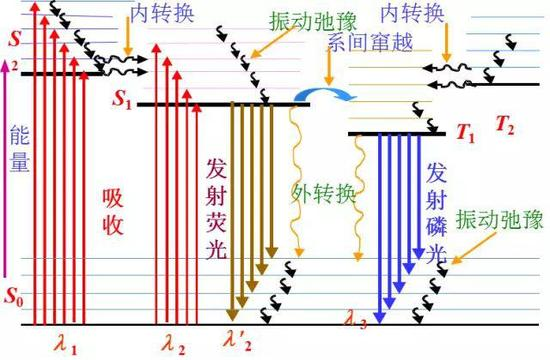
\includegraphics[width=0.6\textwidth]{fluoresence.jpg}
\caption*{荧光、磷光能级跃迁示意图}
\end{figure}
\end{frame}

\begin{frame}[t]\frametitle{含时演化精确解:离散变量表象(DVR)}
\begin{itemize}
	\item 解决含时薛定谔方程:$\hat{H} \psi(x;t) = i \hbar \frac{\partial}{\partial t} \psi(x;t)$
	\item 将波函数离散化——表现为每一个格点上的数值
	\item 将哈密顿量转化为一个矩阵,波函数转化为列向量
	\item 缺点:格点数庞大,计算量随维度呈指数上升
	\begin{equation*}
	\tiny
	\hat{H} \rightarrow
	\begin{pmatrix}
	1 & 0.5 \\
	0.5 & 1
	\end{pmatrix}
	, \quad
	\psi(x) \rightarrow
	\begin{pmatrix}
	1 \\
	0
	\end{pmatrix}
	\end{equation*}
\end{itemize}


\begin{figure}
\centering
\subfigure{
	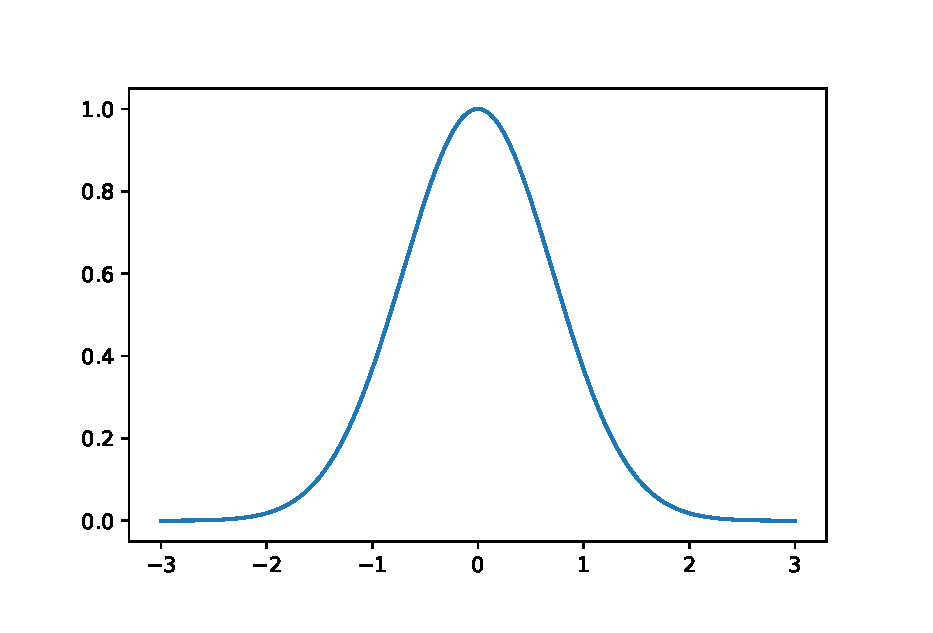
\includegraphics[width=0.4\textwidth]{gaussian_continuous.eps}
}
\subfigure{
	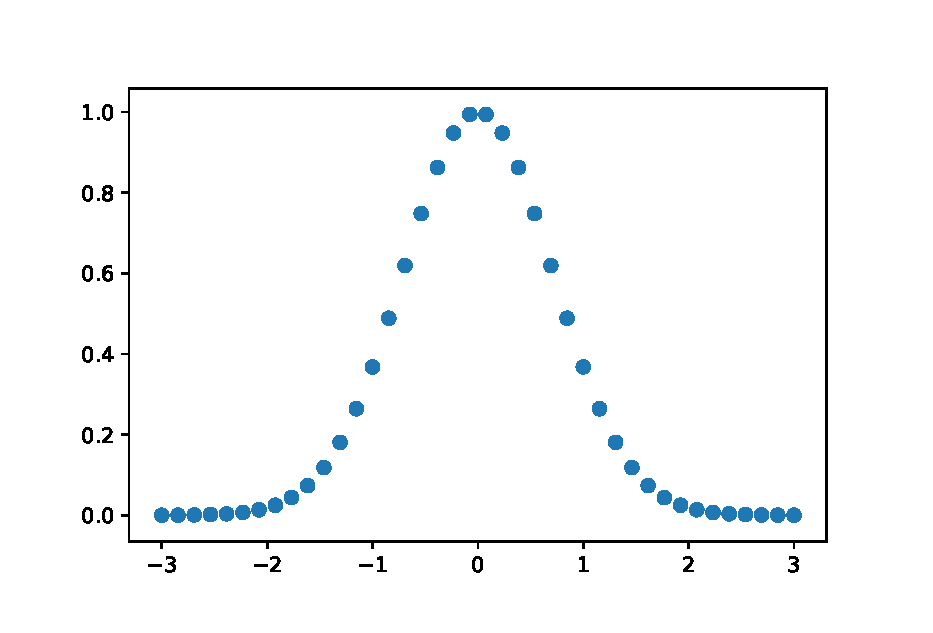
\includegraphics[width=0.4\textwidth]{scattered_gaussian.eps}
}
\end{figure}
\end{frame}

\begin{frame}[t]\frametitle{半经典量子动力学:保留一部分量子修正}
级数展开:
\begin{equation*}
\frac{\pi^2}{6} = \underbrace{\overbrace{\frac{1}{1^2} + \frac{1}{2^2}}^\text{经典力学(1.25)} + \overbrace{\frac{1}{3^2} + \frac{1}{4^2}}^\text{一阶修正(0.1736)} + \overbrace{\frac{1}{5^2} + \frac{1}{6^2} +\frac{1}{7^2} + \frac{1}{8^2}}^\text{二阶修正(0.1038)} + \,...}_\text{量子精确解 ($\sim$ 1.6449)}
\end{equation*}
动力学演化(磨雅括号):
\begin{equation*}
\small
\begin{aligned}
	 &\{\{A, H\}\}=\frac{2}{\hbar} A \sin \left[\frac{\hbar}{2}\left(\sum_{i} \overleftarrow{\partial}_{q_{i}} \overrightarrow{\partial}_{p_{i}}-\overleftarrow{\partial}_{p_{i}} \overrightarrow{\partial}_{q_{i}}\right)\right] H  \rightarrow \text{量子精确解} \\
	 &=\underbrace{\{A, H\}}_\text{经典力学}+\underbrace{\sum_{j=1}^{\infty} \frac{(-1)^{j}}{(2 j+1) !}\left(\frac{\hbar}{2}\right)^{2 j} A\left[\sum_i\left(\overleftarrow{\partial}_{q_{i}} \overrightarrow{\partial}_{p_{i}}-\overleftarrow{\partial}_{p_{i}} \overrightarrow{\partial}_{q_{i}}\right)^{2 j+1}\right] H}_\text{各阶修正}
\end{aligned}
\end{equation*}
\end{frame}


\section{半经典磨雅动力学}
\begin{frame}[t]\frametitle{特点}
半经典磨雅动力学(Semiclassical Moyal Dynamics, SMD)
\begin{itemize}
	\item 任意调整量子修正的阶数
	\item 推导高阶动力学方程方法简洁,易操作
\end{itemize}
\begin{figure}
\centering
\subfigure{
	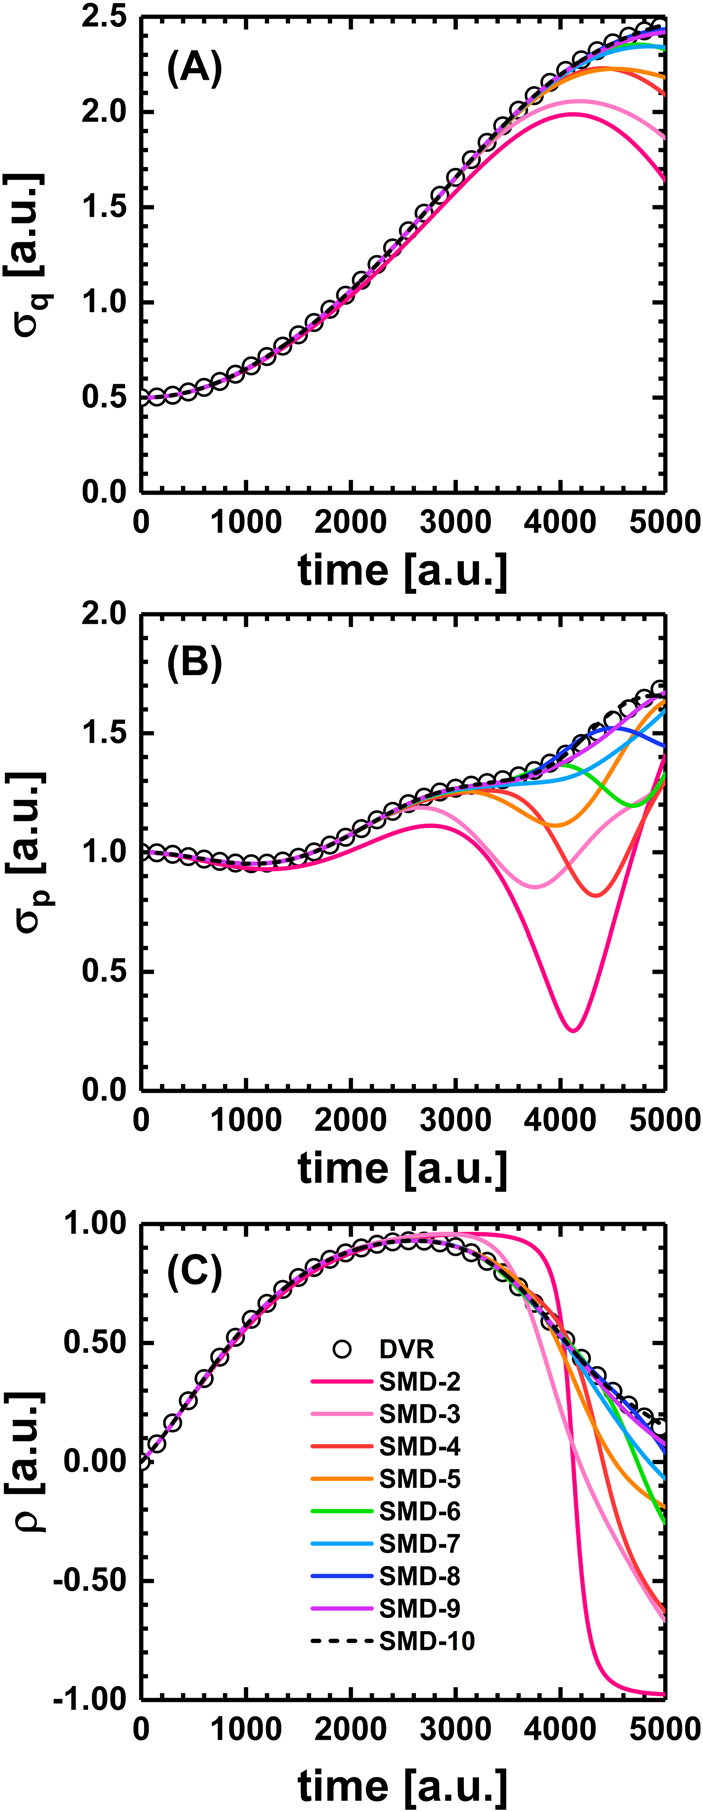
\includegraphics[height=0.32\textheight]{a4.png}	
}
\subfigure{
	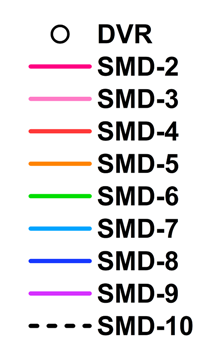
\includegraphics[height=0.32\textheight]{SMD-minimal.png}
}
\caption*{不同阶数的SMD演化\blankfootnote{\tiny SHEN Y, WANG L. Semiclassical Moyal dynamics[J/OL]. The Journal of Chem­ical Physics, 2018, 149(24): 244113}}
\end{figure}
\end{frame}

\begin{frame}[t]\frametitle{存在问题}
\begin{itemize}
 \item 稳定性差,容易发生数值崩溃\blankfootnote{\tiny 顾锴. 相空间哈密尔顿动力学的稳定性研究[D]. 杭州: 浙江大学, 2019.}
 \item 使用单中心高斯分布描述相空间分布——无法处理多中心相空间分布
\end{itemize}
\begin{figure}
\subfigure{
	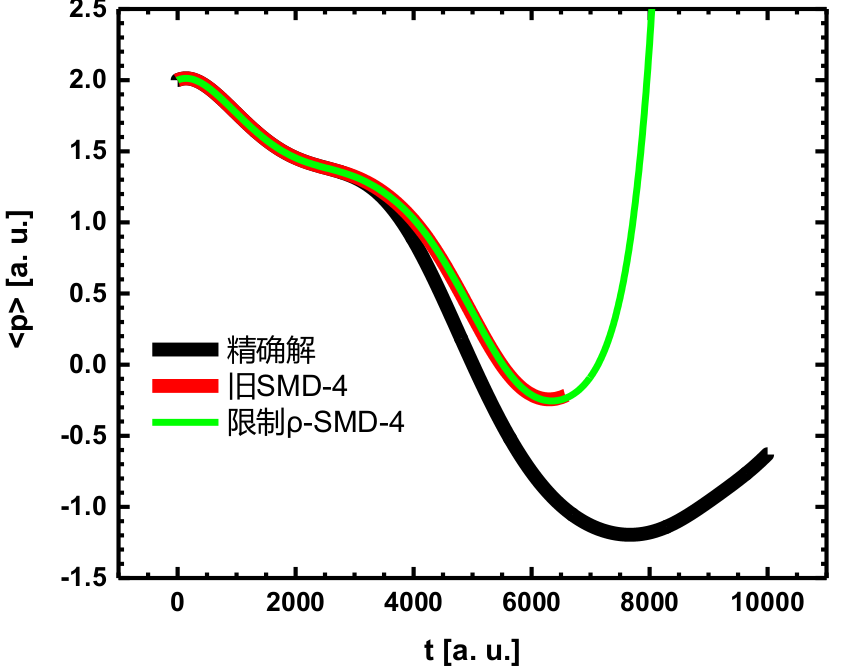
\includegraphics[height=0.42\textheight]{SMDcollapse.png}
}
\subfigure{
	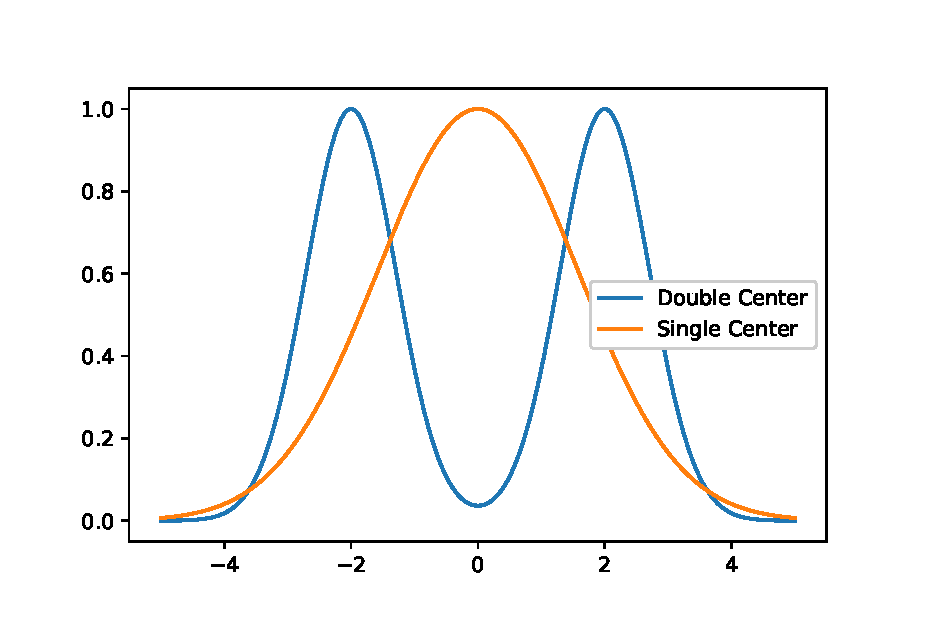
\includegraphics[height=0.42\textheight]{centers_gaussian.eps}
}
\end{figure}

\end{frame}
\section{主要研究内容}

\begin{frame}[t]\frametitle{技术路线}
\vfill
\begin{itemize}
	\item Classical-Wigner分布:对实空间下的波函数使用Wigner变换得到的相空间分布
	\item 将相空间分布格点化作为无相互作用的粒子
	\item 计算每个粒子受到的力,进行演化
\end{itemize}

\begin{figure}
\subfigure{
	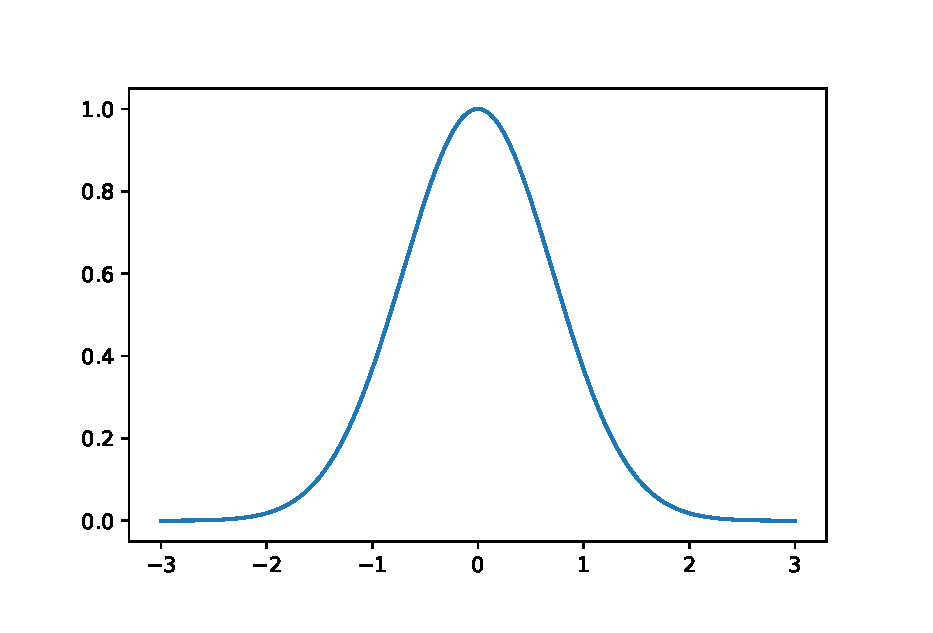
\includegraphics[width=0.3\textwidth]{gaussian_continuous.eps}
}
\subfigure{
	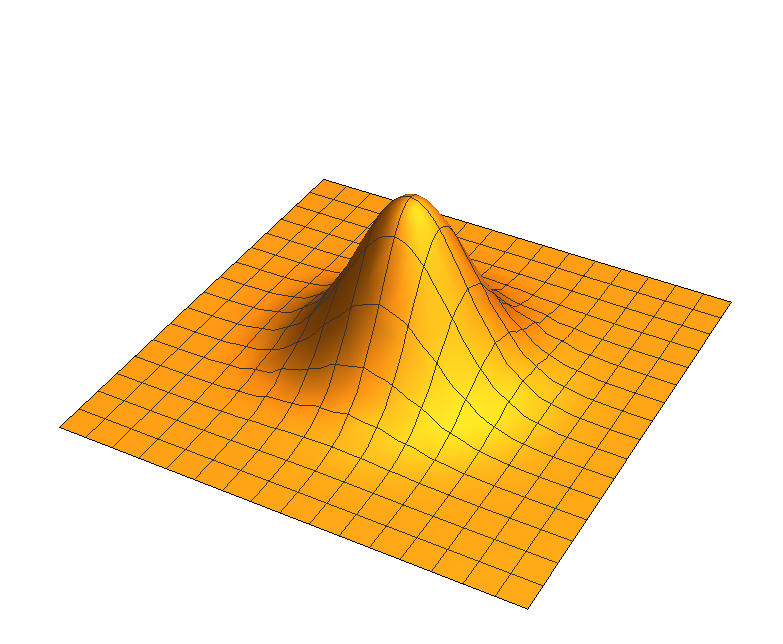
\includegraphics[width=0.3\textwidth]{2gaussian_continuous.eps}
}
\subfigure{
	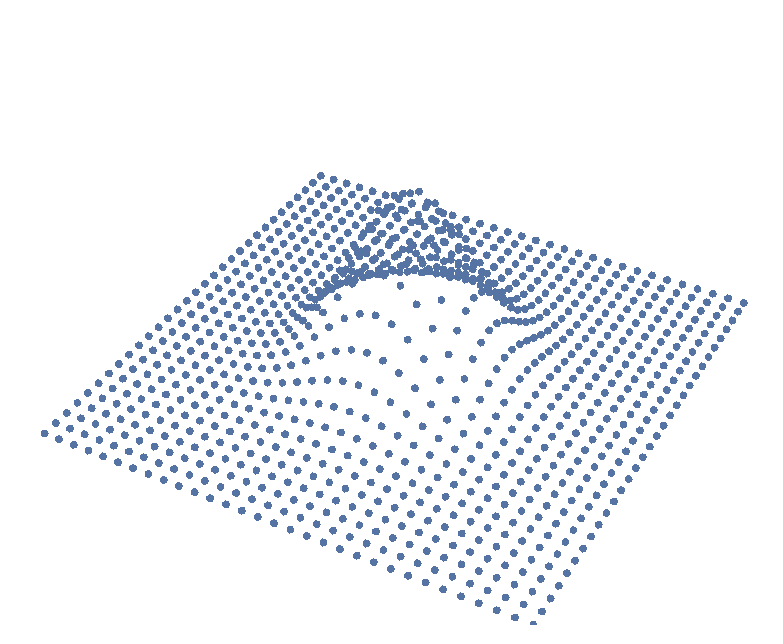
\includegraphics[width=0.3\textwidth]{2gaussian_discrete.eps}
}
\end{figure}


\end{frame}

\begin{frame}[t]\frametitle{Classical-Wigner分布下的分子动力学模拟}
\vfill
\begin{figure}
\subfigure{
	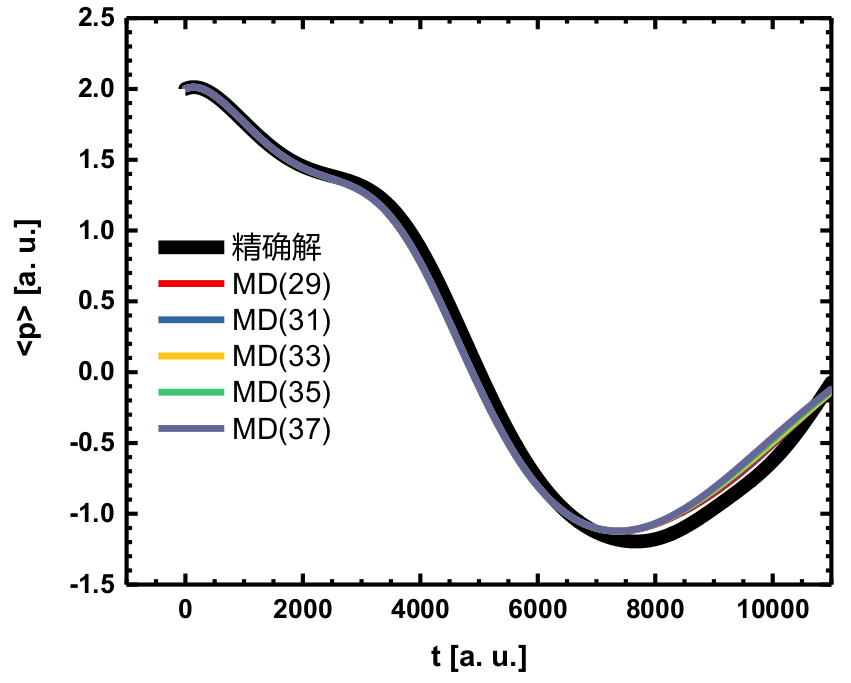
\includegraphics[width=0.45\textwidth]{md_kaigu.png}\blankfootnote{\tiny 顾锴. 相空间哈密尔顿动力学的稳定性研究[D]. 杭州: 浙江大学, 2019.}
}
\subfigure{
	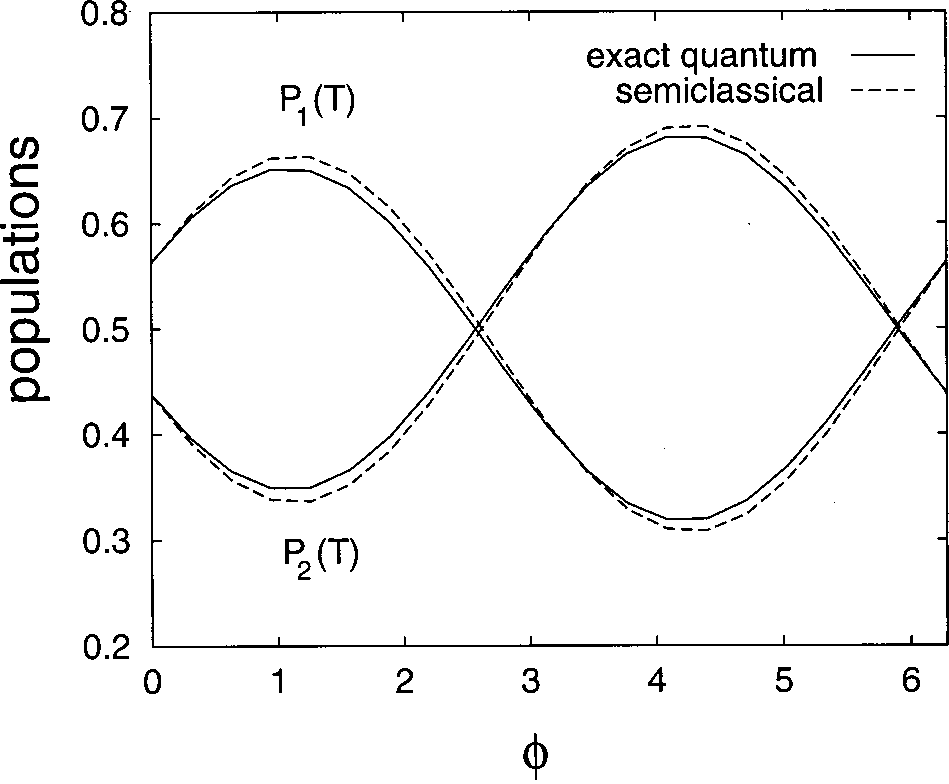
\includegraphics[width=0.45\textwidth]{md_Martens.png}
}
\end{figure}
\end{frame}

\begin{frame}[t]\frametitle{引入SMD修正}
\vfill
\begin{itemize}
	\item 每个粒子由狄拉克函数表达:$\delta(x-x_0)\delta(p-p_0)$
	\item $dt$时间演化后与实际期望值演化的差别:
\begin{equation*}
\begin{cases}
	D(x^2) = p_0^2 dt \\
	D(x p) = - x_0 p_0 dt \\
	D(p^2) = x_0^2 dt
\end{cases}
\end{equation*}
	\item 使用SMD框架修正误差:
	\begin{equation*}
		\delta(x-x_0)\delta(p-p_0) \rightarrow \mathbf{?}
	\end{equation*}
\end{itemize}
\end{frame}

\begin{frame}[t]\frametitle{计划、预期目标}
计划:
\begin{itemize}
	\item 2020年2月:完成基于粒子化Wigner变换的半经典磨雅动力学的关键公式的推导;
	\item 2020年3月:基于粒子化Wigner变换的半经典磨雅动力学的主要框架;
	\item 2020年4月:完成程序,对标准一维模型进行测试,分析程序运行情况及修正方法;
	\item 2020年5月:优化修正方法;若能够保证数值稳定性与结果的可靠性,对多维模型进行测试。
\end{itemize}
预期目标:
\begin{itemize}
\item 研究出基于粒子化相空间分布的SMD方法的一般方法;
\begin{itemize}
\item 提高SMD方法的稳定性;
\item 相较经典分子动力学模拟有更高的精度。
\end{itemize}
\end{itemize}
\end{frame}
\end{document}